\chapter{LabVIEW VI}

\begin{figure}[h]
\centering 
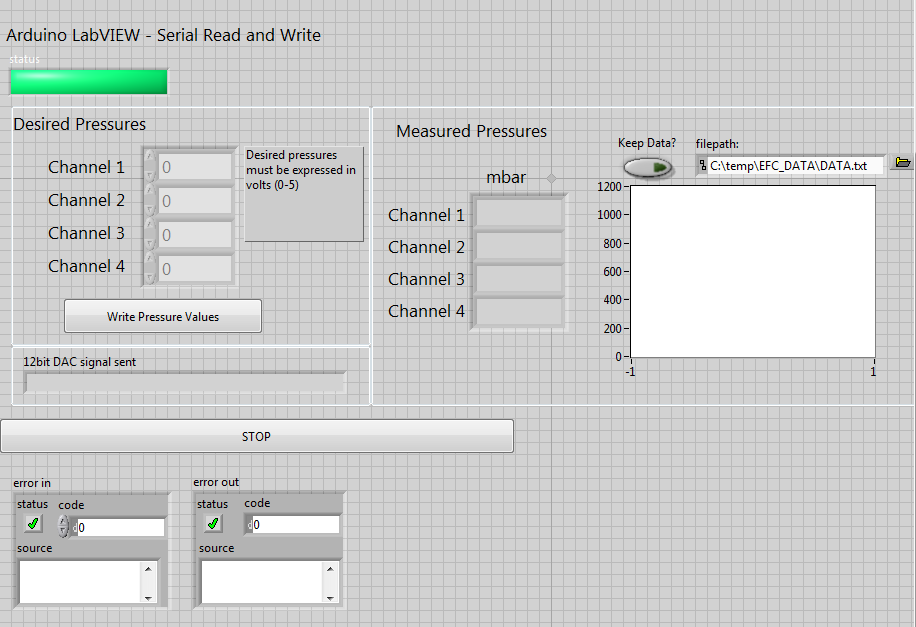
\includegraphics[width=1.0\columnwidth]{frontend.PNG} 
\caption[LabVIEW Frontend]{LabVIEW Frontend} 
\label{fig:frontend} 
\end{figure}

\begin{figure}[h]
\centering 
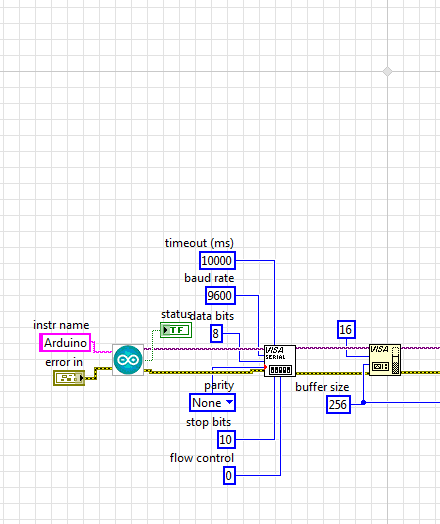
\includegraphics[width=0.60\columnwidth]{backend11.PNG} 
\caption[LabVIEW Backend 1]{LabVIEW Backend 1 } 
\label{fig:backend11} 
\end{figure}

\begin{figure}[h]
\centering 
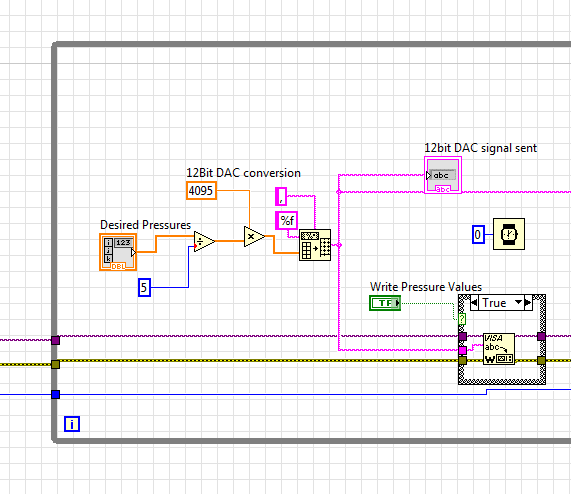
\includegraphics[width=0.60\columnwidth]{backend12.PNG} 
\caption[LabVIEW Backend 2]{LabVIEW Backend 2} 
\label{fig:backend12} 
\end{figure}

\begin{figure}[h]
\centering 
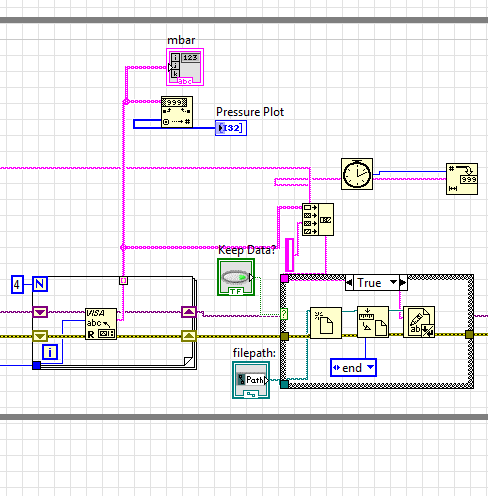
\includegraphics[width=0.60\columnwidth]{backend13.PNG} 
\caption[LabVIEW Backend 3]{LabVIEW Backend 3} 
\label{fig:backend13} 
\end{figure}

\begin{figure}[h]
\centering 
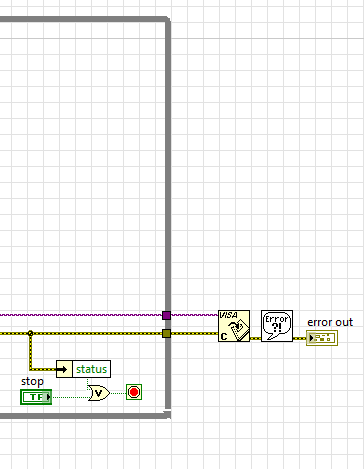
\includegraphics[width=0.60\columnwidth]{backend14.PNG} 
\caption[LabVIEW Backend 4]{LabVIEW Backend 4} 
\label{fig:backend14} 
\end{figure}
